\documentclass[12pt]{article}
\usepackage{fancyhdr, amsmath, amsthm, amssymb, mathtools, lastpage}
\usepackage[margin=0.7in, top=1in,bottom=1in]{geometry}
\newcommand{\scinot}[2]{#1\times10^{#2}}
\newcommand{\bra}[1]{\left<#1\right|}
\newcommand{\ket}[1]{\left|#1\right>}
\newcommand{\dotp}[2]{\left<\left.#1\right|#2\right>}
\newcommand{\rd}[2]{\frac{d#1}{d#2}}
\newcommand{\pd}[2]{\frac{\partial#1}{\partial#2}}
\newcommand{\rtd}[2]{\frac{d^2#1}{d#2^2}}
\newcommand{\ptd}[2]{\frac{\partial^2 #1}{\partial#2^2}}
\newcommand{\norm}[1]{\left|\left|#1\right|\right|}
\newcommand{\abs}[1]{\left|#1\right|}
\newcommand{\pvec}[1]{\vec{#1}^{\,\prime}}
\newcommand{\tensor}[1]{\overleftrightarrow{#1}}
\let\Re\undefined
\let\Im\undefined
\DeclareMathOperator{\Re}{Re}
\DeclareMathOperator{\Tr}{Tr}
\DeclareMathOperator{\Im}{Im}
\newcommand{\expvalue}[1]{\left<#1\right>}
\usepackage[labelfont=bf, font=scriptsize]{caption}
\usepackage{tikz}
% \usepackage[version=3]{mhchem}
% \usepackage{hyperref}
\usepackage{enumerate}
% \usepackage{graphicx}
% \usepackage{setspace}
\everymath{\displaystyle}

\begin{document}

\pagestyle{fancy}
\rhead{Yubo Su --- Cliff class woohoo!}
\cfoot{\thepage/\pageref{LastPage}}

\title{Ph125c Private Final Review Session Note --- v. 1.4}
\author{Yubo, Cassidy, Paul, Chien-Yi}
\date{06/01/2014}

\maketitle

\tableofcontents

\section{Changelog}

\begin{itemize}
    \item 06/07/14 --- 1.4 --- Changed explanation of ``self interaction'' in phonon section.
    \item 06/05/14 --- 1.3 --- Fixed a few odd typos, added a few footnotes and parenthetical remarks about intuition.
    \item 06/03/14 --- 1.2 --- Added blurb from Politzer conversation about crystals, pointed out that Higgs boson/the like are actually quantum fields.
    \item 06/01/14 --- 1.1 --- Tried yet again (unsuccessfully) to explain a bit more about what a quantum field is.
    \item 05/29/14 --- 1.0 --- Day of review session!
\end{itemize}
\section{Yubo --- Ahranov-Bohm, Dirac charge quantization}

\subsection{Ahranov-Bohm effect derivation}

We first ask what happens quantum mechanically when we introduce a magnetic field to a quantum mechanical system. Let's start with the electromagnetic Lagrangian
\begin{align}
    L = \frac{m}{2}\left( \rd{\vec{r}}{t} \right)^2 + \frac{q}{c}\rd{\vec{r}}{t} \cdot \vec{A} - q\phi
\end{align}

We will now specialize to the Ahranov-Bohm effect. Exhibit $\phi = 0$ and $\vec{A}$ such that the setup in Figure \ref{AB} is satisfied.

\begin{figure}[!h]
    \centering
    \begin{tikzpicture}[scale=0.5]
        \filldraw(-8,0) circle(0.8pt);
        \node[left, above] at (-8,0.3) {Source};
        \draw[ultra thick] (0,5) -- (0,2.3);
        \draw[ultra thick] (0,2) -- (0,-2);
        \draw[ultra thick] (0,-5) -- (0,-2.3);
        \draw[thick] (8,5) -- (8,-5);
        \node[right] at (5,5) {Screen};
        \draw[dashed, ->] (-8,0) -- (0,2.2);
        \draw[dashed, ->] (0,2.2) -- (8,0);
        \node[above] at (-3,1.7) {$P_1$};
        \draw[dashed, ->] (-8,0) -- (0,-2.2);
        \draw[dashed, ->] (0,-2.2) -- (8,0);
        \node[below] at (-3,-1.7) {$P_2$};
        \draw(1.5,0) circle(25pt);
        \node at (1.5,0) {{\tiny $\vec{B} \neq 0$}};
    \end{tikzpicture}
    \caption{Ahranov-Bohm setup}
    \label{AB}
\end{figure}

Now let's compare the propagators over the two paths $P_1, P_2$, which by path integral formulation goes like $U \sim \exp\left[ \frac{i}{\hbar}\int L[x(t)]\; dt \right]$. 

Let's focus on the contribution by the magnetic field itself, to see how it changes the classical two-slit diffraction pattern. We note that the phase change of $U$ due to $\vec{B}$ over the path $P_1$ and $P_2$ respectively are given by
\begin{align}
    \psi_1 &\sim \exp\left[ \frac{i}{\hbar}\int\limits_{P_1} L[x(t)]\;dt \right] & \psi_2 &\sim \exp\left[ \frac{i}{\hbar}\int\limits_{P_2} L[x(t)]\;dt \right]\\
    &\sim \psi_{1,0}\exp\left[ -\frac{iq}{\hbar c} \int\limits_{P_1}d\vec{r} \cdot \vec{A} \right] & &\sim \psi_{2,0}\exp\left[ -\frac{iq}{\hbar c} \int\limits_{P_2}d\vec{r} \cdot \vec{A} \right]
\end{align}
with $\psi_{i,0}$ the initial wavefunction in the absence of $\vec{B}$. We can then write down the total wavefunction seen on the screen at each point as
\begin{align}
    \psi &= \psi_1 + \psi_2\\
    &= \psi_{1,0}\exp\left[ -\frac{iq}{\hbar c} \int\limits_{P_1}d\vec{r} \cdot \vec{A} \right] + \psi_2 \left[ -\frac{iq}{\hbar c} \int\limits_{P_2}d\vec{r} \cdot \vec{A} \right]
\end{align}
but then since the overall wavefunction can be changed up to a phase we can factor out one phase and obtain
\begin{align}
    \psi &= \psi_{1,0}\exp\left[ -\frac{iq}{\hbar c} \left(\int\limits_{P_1}d\vec{r} \cdot \vec{A}  - \int\limits_{P_2}d\vec{r} \cdot \vec{A}\right) \right] + \psi_2\\
    &= \psi_{1,0}\exp\left[ -\frac{iq}{\hbar c} \oint\limits_{P}d\vec{r} \cdot \vec{A} \right] + \psi_2\\
    \text{{\scriptsize (Stokes Theorem)}}&= \psi_{1,0}\exp\left[ -\frac{iq}{\hbar c} \iint\limits_{S(P)}\underbrace{\vec{\nabla} \times \vec{A}}_{\vec{B}} \;dS \right] + \psi_2\\
    &= \psi_{1,0}\exp\left[ -\frac{iq}{\hbar c} \Phi_B \right] + \psi_2\label{ABfin}
\end{align}
where we define the closed path $P = P_1 - P_2$ and $\Phi_B$ is the total magnetic flux through the loop $P$. This shows that the magnetic field, through which the trajectories $P_1, P_2$ do not pass.

One easy way to interpret this result, albeit incorrectly, is to say ``well, the particle does take trajectories that pass through the field, because they travel all possible paths, so it's not surprising the field is detected.'' In fact, if we put an infinite potential barrier around the $\vec{B}$ field such that the particle cannot take any path that goes through the $\vec{B}$ field, the above results still hold!

The Ahranov-Bohm effect is just a byproduct of nonlocality of QM. Below in Figure \ref{ABFig} is an illustration of the two-slit diffraction pattern before/after introduction of a $\vec{B}$ field
\begin{figure}[!h]
    \centering
    \includegraphics[scale=0.4]{Ph125c_AB.png}
    \caption{Picture I found online to help visualise the Ahranov-Bohm effect}
    \label{ABFig}
\end{figure}

\subsection*{Dirac charge quantization}

Let's examine carefully \eqref{ABfin}. If it just so happens that $\Phi_B = \frac{2n\hbar c\pi}{q}$ then the exponent goes like $e^{-i2\pi}$ and suddenly the Ahranov-Bohm effect vanishes for these specific values of $\Phi_B$. We call $\Phi_0 = \frac{2\hbar c\pi}{q}$ the \emph{flux quantum} (so any integral multiple of the flux quantum is undetectable by Ahranov-Bohm).

This leads us to a peculiar construction called the \emph{Dirac string}. If we construct a long solenoid of vanishing radius, and fix the current exactly correctly such that $\Phi_B = n\Phi_0$ then we will effectively observe two magnetic monopoles at either end of the solenoid. If we then assume that magnetic monopoles obey Gauss's Law for magnetic charge $\vec{\nabla} \cdot \vec{B} = 4\pi\rho_m \neq 0$, then we can compute the allowed values of these magnetic monopoles by matching the flux through an arbitrary surface due to such a ``monopole'' to the entering flux through the infinitisemal Dirac string. In other words, we can set up the following sort of construction Figure \ref{DiracConst}.
\begin{figure}[!h]
    \centering
    \begin{tikzpicture}[scale=0.5]
        \filldraw(-5,0) circle(3pt);
        \node[below] at (-5,0) { {\tiny $q_m$}};
        \draw[dotted,<-] (0,0) -- (-5,0);
        \node[below] at (0,0) { {\tiny Dirac String}};
        \draw[dashed] (-5,0) circle(2);
        \node[below, right] at (-3.6,-1.4) { {\tiny$S$}};
    \end{tikzpicture}
    \caption{Dirac charge quantization setup. Note the small dotted line is the Dirac string, and the dashed surface $S$ is the surface over which we can apply Gauss's Law.}
    \label{DiracConst}
\end{figure}

This might be a little bit confusing, so let's just clarify this: \emph{we are not postulating the existence of these monopoles; we are saying if monopoles were sourced by the undetectable Dirac String then the resulting condition quantizes the ``monopole'' that we think we're seeing}. 

We note that the flux entering the Gaussian surface (due to Dirac string) is $n\Phi_0$ while the flux leaving the surface (due to the hypothetical monopole) is 
\begin{align}
    \iint \vec{B} \cdot \hat{n} \;dS &= \iiint \vec{\nabla} \cdot \vec{B} \;dV\\
    &= 4\pi q_m
\end{align}
which shows that $q_m = \frac{n\Phi_0}{4\pi} = n\frac{\hbar c}{2q}$. Note that since Dirac strings are completely unobservable, this shows that if monopoles were to ever exist they would have to come in integer multiples of $\frac{\hbar c}{2e}$ with $e$ the quantized electric charge.

\section{Cassidy --- Superconductors, confinement, Josephson junctions}

\subsection{Superconductors}
At low temperatures, two electrons come together and form \emph{Cooper pairs} that act like bosons. This leads us to guess that the probability goes with the charge, i.e. $\psi^\dagger\psi \sim \rho$, or that the current $\rd{\rho}{t}$ goes with the probability current. More quantitatively, we can write using the  continuity equation
\begin{align}
    \rd{\rho}{t} + \vec{\nabla} \cdot \vec{J} &= 0\\
    \rd{}{t}\left( \psi^\dagger \right)\psi + \psi^\dagger\pd{\psi}{t} + \vec{\nabla} \cdot \vec{J}&= 0
\end{align}

We then plug in the SE for a $\psi$ in the presence of some electromagnetic field, which looks like $i\hbar \pd{}{t}\psi = \left[ \frac{\left( P - \frac{q}{c}A \right)^2}{2m} + q\phi \right]\psi$, and plugging this into our above equation and take care of some algebra to find (we can check this by taking divergence of this expression)
\begin{align}
    \vec{J} &= \frac{1}{2}\left[ \left( \frac{-i\hbar \nabla - \frac{q}{c}A}{m} \psi\right)^\dagger\psi + \psi^\dagger\left( \frac{-i\hbar \nabla - \frac{q}{c}A}{m} \right)\psi \right]
\end{align}

Then if we plug in the ansatz $\psi = \sqrt{\rho(\vec{r},t)}e^{i\theta(\vec{r},t)}$ to the above\footnote{This is just our previous ansatz but allowing the phase to vary; note that this doesn't change the validity of our earlier calculations because any phase would have cancelled.} and make the electrostatic approximation we magically end up with (the actual algebra is covered in my actual class notes; we skipped it for the review session)
\begin{align}
    \Box^2\vec{A} &= -\lambda^2\vec{A} & \lambda^2 &= \frac{\mu_0\rho q}{mc}
\end{align}

Then if we try to plug in an incident wave $\vec{A} \sim e^{\alpha \mathbf{k} \cdot \mathbf{x}}$, then we find that there are only two solutions in the superconductor, $\vec{A} \sim e^{\pm \lambda x}$, and we know that the growing one is unphysical so we know that the fields must be attenuated upon penetration into the superconductor.

\subsection{Meissner effect, rederivation flux quantization condition}

We then note the Meissner effect, where at low temperatures fields are expelled from superconductors. Then if we try the construction where we send a $\vec{B}$ field into a ring, then we can get it so that that the field goes through both the middle and the outside of the ring. The cool thing then is if we turn off the magnetic field, the field in the middle remains \emph{trapped} because the field lines cannot go through the superconductor to vanish (sorry, this would make a lot more sense with diagrams). 

We can rederive the flux quantization condition using this setup. Recall that we made the ansatz $\psi = \sqrt{\rho}e^{i\theta}, \vec{J} = \frac{\hbar}{m}\rho\left[ \vec{\nabla}\theta - \frac{q}{\hbar c}\vec{A} \right] = 0$. If we then take the line integral of both sides of the above equation we find
\begin{align}
    \frac{\hbar c}{q}\oint \vec{\nabla} \theta \cdot d\vec{r} &= \oint \vec{A} \cdot d\vec{r}\\
    &= \iint \vec{\nabla} \times \vec{A} dS\\
    &= \Phi_B
\end{align}

Noting then that the right hand side must be an integral multiple of $2\pi$: line integral of $\vec{\nabla}\theta$ which is just $\theta$ evaluated at the endpoints (note $\theta$ is periodic and multivalued!) then by periodicity conditions we have that the line integral must go like $2\pi n$. Then we recover $\Phi_B = \frac{2\pi n\hbar c}{q}$. 

\subsection{Confinement}

Let's then put two magnetic monopoles inside a superconducting material (connect them with Dirac strings to far away outside the superconductor). We then find that the only allowed field, because superconductors expel fields, is the shortest path between the two, i.e. a straight line\footnote{This was not presented very convincingly in class, but I thought of it this way: you must have some field lines due to the potential difference, and in the superconductor there is an infinite penalty for deviating from the shortest path as the field attenuates infinitely.}. This shortest path of $\vec{B}$ then forms a \emph{flux tube} of concentrated magnetic flux. We then find that the energy stored within this flux tube goes something like $E \sim TL$ with $T$ some sort of \emph{tension} and $L$ the length of the string\footnote{This was also stated without proof in class, but the reason this is true is because the magnetic field within the flux tube cannot vary with length: length is continuous while the flux through the flux tube is discrete/quantized, so elongating the string by some tiny amount cannot change the field, repeat ad infinitum.  So energy goes linearly with length.}. Then the energy increases unboundedly with length, and it becomes energetically efficient to spawn additional particles than to keep increasing the length of the flux tube. The fact that we cannot separate magnetic monopoles is related to this effect, and it is called \emph{confinement}; it also applies to quarks!

\subsection{Josephson Junctions}
Let's now look at Josephson Junctions and figure out what happened. How Josephson junctions look is depicted in Figure \ref{JJ}
\begin{figure}[!h]
    \centering
    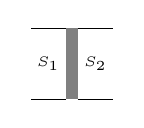
\begin{tikzpicture}[scale=0.3]
        \fill[gray] (-0.25,-1.5) rectangle(0.25,1.5);
        \draw (-0.25,-1.5) -- (-1.75,-1.5);
        \draw (-0.25,1.5) -- (-1.75,1.5);
        \node at (-1,0) { {\tiny$S_1$}};
        \node at (1,0) { {\tiny $S_2$}};
        \draw (0.25,1.5) -- (1.75,1.5);
        \draw (0.25,-1.5) -- (1.75,-1.5);
    \end{tikzpicture}
    \caption{One Josephson Junction}
    \label{JJ}
\end{figure}

We then represent the wavefunction within either superconductor to be $\psi_1, \psi_2$, such that the total wavefunction looks like
\begin{align}
    \ket{\psi} = \begin{bmatrix} \psi_1\\ \psi_2 \end{bmatrix} 
\end{align}
and some interaction Hamiltonian that acts on the system that looks of form
\begin{align}
    H &= \begin{bmatrix} H_1 & \kappa \\ \kappa^* & H_2 \end{bmatrix} 
\end{align}

If we then plug in our previous ansatz $\psi_1 = \sqrt{\rho_1}e^{i\theta_1}, \psi_2 = \sqrt{\rho_2}e^{i\theta_2}$ along with the assumption that $\rho_1 = \rho_2$ (connected conductors) through the SE we can wade through some algebra and find
\begin{align}
    \vec{J} &= J_0\sin\left( \delta + \frac{q}{\hbar}\int\limits_{}^{t}V(t')\;dt' \right)
\end{align}

{\em Yubo's note: $V$ is the voltage between the two nodes, and $\delta$ is the phase shift between the two. The algebra is covered in the full class notes}

The awesome part is that the current never fully vanishes!

Let's consider a full blown Josephson Junction, like in Figure \ref{JJ2}
\begin{figure}[!h]
    \centering
    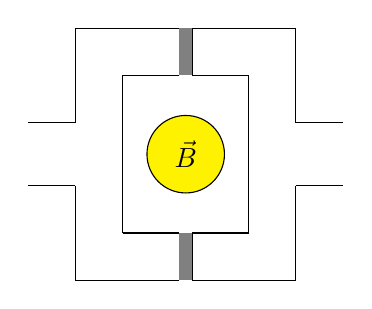
\begin{tikzpicture}[scale=0.2]
        \draw (-10,2) -- (-7,2);
        \draw (-7,2) -- (-7,8);
        \draw (-7,8) -- (-0.4,8);
        \draw (-0.4,8) -- (-0.4,5);
        \draw (-0.4,5) -- (-4,5);
        \draw (-4,5) -- (-4,-5);
        \draw (4,5) -- (4,-5);
        \draw (10,2) -- (7,2);
        \draw (7,2) -- (7,8);
        \draw (0.4,8) -- (0.4,5);
        \draw (0.4,5) -- (4,5);
        \draw (7,8) -- (0.4,8);
        \draw (-10,-2) -- (-7,-2);
        \draw (-7,-2) -- (-7,-8);
        \draw (-7,-8) -- (-0.4,-8);
        \draw (-0.4,-8) -- (-0.4,-5);
        \draw (-0.4,-5) -- (-4,-5);
        \draw (10,-2) -- (7,-2);
        \draw (7,-2) -- (7,-8);
        \draw (0.4,-8) -- (0.4,-5);
        \draw (0.4,-5) -- (4,-5);
        \draw (7,-8) -- (0.4,-8);
        \filldraw[yellow, draw=black] (0,0) circle(70pt);
        \node at (0,0) {$\vec{B}$};
        \fill[gray] (-0.4,5) rectangle(0.4,8);
        \fill[gray] (-0.4,-5) rectangle(0.4,-8);
    \end{tikzpicture}
    \caption{Double Josephson Junction. Grey sections are insulators, yellow (woohoo, color!) is the magnetic field.}
    \label{JJ2}
\end{figure}

The phase shift along the top path then goes something like $\delta_1 + \frac{q}{\hbar c}\int\limits_{P_1} \vec{A} \cdot d\vec{r}$ and the bottom path $\delta_2 + \frac{q}{\hbar c}\int \limits_{P_2}\vec{A} \cdot d\vec{r}$. This allows us to see the phase shift of the currents and thus measure $\vec{B}$ super accurately (think interferometers!).

\section{Paul --- Quantum Hall effect, Crystals}

\subsection{Quantum Hall Effect (missing punch line)}

Let's start with a thin sheet in the $xy$ plane, exhibit a $\vec{B} = B\hat{z}$ field, and Hamiltonian $H = \frac{\left( \vec{p} - \frac{q}{c}\vec{A} \right)}{2m}$. This produces a vector potential $\vec{A} = \frac{B}{2}\left( -y,x,0 \right)$. This then gives us Hamiltonian
\begin{align}
    H &= \frac{1}{2m}\left( p_x + \frac{qB}{2c}y, p_y - \frac{qB}{2c}x \right)^2\\
    &= \frac{P_s^2}{2m} + \frac{1}{2}m\omega_0^2 Q_s^2
\end{align}
where we define $P_s = P_y - \frac{qxB}{2c}, Q_s = \left(cP_{x} + \frac{qyB}{2}\right)\frac{1}{qB}, \omega_0 = \frac{qB}{mc}$, where if we compute out the commutators we find that $P_s, Q_s$ are canonical. Then it is clear that $H$ looks like a 1D quantum harmonic oscillator with some energy $E = \frac{2n + 1}{2}\hbar \omega_0$. 

We can define then creation/annihilation operators for the system, 
\begin{align}
    a^\dagger &= \left( \frac{m\omega_0}{2\hbar} \right)^{1/2}Q_s + i\left( \frac{1}{2m\omega_0\hbar} \right)^{1/2}P_s\\
    &= \left( \frac{c}{2\hbar qB} \right)^{1/2} \left[ \left( P_x + iP_y \right) - i\frac{qB}{2c}\left( x + iy \right) \right]\\
    &= \left( \frac{c}{2\hbar qB} \right)^{1/2} \left[ -i\hbar\left( \pd{}{x} + i\pd{}{y} \right) - i\frac{qB}{2c}\left( x + iy \right) \right]
\end{align}
where we go to coordinate space. But then it seems quite natural that we should introduce $z = x + iy$, for which we know that $\pd{}{z^*} = \frac{1}{2}\left( \pd{}{x} + i\pd{}{y} \right)$, which would then take us to
\begin{align}
    a^\dagger\ket{0} &= \left\{ 2\hbar \pd{}{z^*} + \frac{qB}{2c}z \right\}\psi_0(z,z^*) = 0
\end{align}

Let's then introduce an ansatz for the ground state $\psi_0 = e^{-\frac{qB}{4\hbar c}\abs{z}^2}U(z,z^*)$. If we then plug this into our above equation we find that $a^\dagger\ket{0} \sim e^{-qB\abs{z}^2/4\hbar c} \pd{}{z^*}U(z,z^*) = 0$, which since the exponent doesn't ever vanish we find that $U(z,z^*) = U(z)$ with $U(z)$ some analytic function of $z$.

Let's instead investigate if we choose a different $\vec{A} = B(0,x,0)$. This then gives our Hamiltonian
\begin{align}
    H &= \frac{P_x^2}{2m} + \frac{1}{2}m\omega^2\left[ X - \frac{P_y}{m\omega_0} \right]^2
\end{align}
so we are effectively shifting the wavefunction by some constant $P_y$, because it doesn't interact with $X, P_x$. So we can then define $X_0 = \frac{P_y}{m\omega_0}$. 

Let's then make our plate $d_x \times d_y$, then our momenta satisfy $P_y = \frac{2\pi \hbar}{d_y}n$ because particle in a box. But so we find that $0 \leq X_0 \leq d_x$. Then if we write $P_y = m\omega_0X_0 = \frac{2\pi \hbar}{d_y}N$ combining our two conditions, then we find that $0 \leq N \leq \frac{m\omega_0 d_x d_y}{2\pi \hbar}$. This then shows that $0 \leq N \leq \frac{BA}{\Phi_0}$ with $\Phi_0$ the flux quantum. We don't know why this is important. 

The farthest we got in this discussion is that each Landau level has degeneracy $\frac{BA}{\Phi_0}$ levels, but we can't figure out what the difference between Landau levels and energy levels, because we showed that $U(z)$ is infinitely degenerate because infinite choice of $U(z)$. Perhaps the way we can look at this is that energy levels are infinitely degenerate because orbits can be translated within the slab of metal, but Landau levels are the translationally invariant energy levels (?) of some sort, of which there arise degeneracies due to the quantization condition of $P_y$ the translational parameter. 

\subsection{Crystals}

If we have some primitive cell that ranges from $0$ to $a+b$ with $V(0 < x < a) = 0, V(a < x < b) = V_0$ the typical crystal cell, then we can write down the propagating solutions (non-bound solutions) as
\begin{align}
    \psi_{1E} &= A_1e^{ik_1x} + B_1e^{-ik_1x} & \psi_{2E} &= A_2e^{ik_2x} + B_2e^{-ik_2x}\label{propsols}
\end{align}
with $k_1 = \sqrt{\frac{2mE}{\hbar}}, k_2 = \sqrt{\frac{2m(E-V_0)}{\hbar}}$ by just solving the SE over both regions.

We first apply the trick of periodicity. Define $c = a+b$ then $\psi(x+c) = \psi(x)$. Then if we write down the translation operator $T = e^{-\frac{i}{\hbar}pc}$ that translates a state by $c$, then we can write down the ansatz $\psi = e^{ikx}U_k(x)$ such that we satisfy $\psi(x) = \psi(x+c)$. 

We can then write down some boundary conditions $\psi_{1E}(0) = \psi_{2E}(0), \psi'_{1E}(0) = \psi'_{2E}(0)$ which also is a condition on $U$, so then if we plug our propagating solutions \eqref{propsols} through these BCs we can bash pretty hard and obtain
\begin{align}
    \frac{k_2^2 - k_1^2}{2k_1k_2}\sinh\left( k_2b \right)\sin\left( k_1a \right) + \cosh(k_2b)\cos(k_1a) &= \cos kc
\end{align}

Then if we plot the left hand side as a function of $E/V_0$ we end up with something that looks roughly like
\begin{figure}[!h]
    \centering
    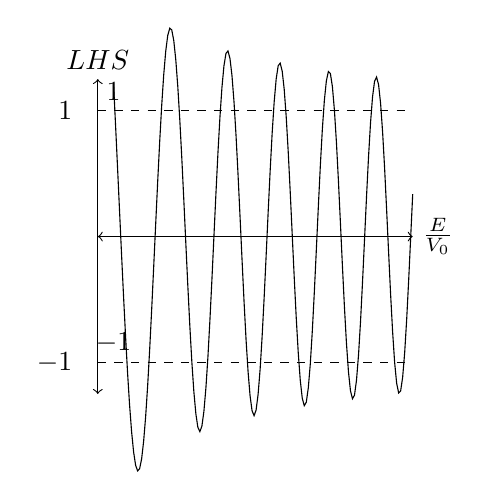
\begin{tikzpicture}[scale=0.2]
        \draw[<->] (0,0) -- (20,0);
        \node[right] at (20,0) {$\frac{E}{V_0}$};
        \draw[<->] (0,-10) -- (0,10);
        \node[above] at (0,10) {$LHS$};
        \draw[dashed] (0,8) -- (20,8);
        \node[right, above] at (1,8) {$1$};
        \node[left] at (-1,8) {$1$};
        \node[right, above] at (1,-8) {$-1$};
        \node[left] at (-1,-8) {$-1$};
        \draw[dashed] (0,-8) -- (20,-8);
        \draw[domain=1:20,samples=150] plot(\x, {cos(deg(\x^(1.2)))*18/\x^(0.2)});
    \end{tikzpicture}
    \caption{Plot of $k,E$}
\end{figure}
where only during the parts where the LHS is within $(-1,1)$ do we have solutions, so this is why we get a band structure in crystals. 

Some interesting problems to solve include a $\sin^2(x)$ potential and replacing the $V_0$ potential from before with a harmonic oscillator potential. 

{\em \small Politzer pointed out that for such periodic potentials particles propagate as if free particles, i.e. no reflection. Intuitively, it's because once the particle reflects off the barrier before it, it reflects back off the barrier behind it and gets to ``try again'' infinitely, and so in the limit all the reflections/transmissions cancel out for perfect transmission. We see this implicitly manifest itself in the assumption that $T$, the translation operator, acts on a wavefunction only by translating it up to a phase.}

{\em \small Note also that just because the particle doesn't reflect doesn't mean it doesn't disperse; since we are dealing with a physical particle $E = \frac{p^2}{2m}$ but at the same time $E \sim \hbar \omega$ and since $p \sim \hbar k$ we see that $\omega \sim k^2$ and the particle propogates dispersively. In other words, if we start a wavepacket inside the periodic potential and send it forward, it will not reflect but it will fatten.}

\section{Yubo --- Klein-Gordon Equation, Dirac Equation, Phonons, QFT}

\subsection{Why the SE sucks}

We know that relativistically time and space should be on equal footing; at most the only symmetry breaking should be that time propagates forward, but otherwise all dynamics should evolve in space and time symmetrically. The Schr\"odinger Equation (henceforth abbreviated SE) sucks at this though; recall the form for $V(x) = 0$
\begin{align}
    i\hbar \pd{\psi(x,t)}{t} &= -\frac{\hbar^2}{2m}\ptd{\psi(x,t)}{x}
\end{align}

This sucks because it's taking two space derivatives and one time derivative. Let's try to fix this.

\subsection{Fixing the SE part 1: Klein-Gordon Equation}

Relativity's real most famous equation is $E^2 = m^2c^4 + p^2c^2$, so this seems like a reasonable jumping off point for the SE. Let's do the typical QM thing and promote everything into operators $E \to H, p \to P$. Then we recall that $H\ket{\psi} = -i\hbar \pd{}{t}\ket{\psi}$ is the SE, so we can plug this in and obtain
\begin{align}
    -\hbar^2 \ptd{}{t}\ket{\psi} &= \left( m^2c^4 - c^2 \hbar^2 \nabla^2 \right)\ket{\psi}\\
    \left(\ptd{}{t} - c^2\nabla^2 + \frac{m^2c^4}{\hbar^2}\right)\ket{\psi} &= 0\label{KG}\\
    \left( \Box^2 + \frac{m^2c^2}{\hbar^2} \right)\ket{\psi} &= 0
\end{align}

\eqref{KG} is the \emph{Klein-Gordon Equation}, but I rewrite it using the \emph{d'Alembertian} to make it even more obviously a relativistic equation. The Klein-Gordon Equation (henceforth the KGE) though runs into many issues, several of which we can examine below
\begin{itemize}
    \item \emph{The first-order SE has been turned into the second-order KGE}, meaning we somehow now need $\psi_0, \dot{\psi}_0$ whereas before we only needed $\psi_0$. This is weird though; where did we suddenly need the extra information? Compared to our usual approach of ``here's a wavefunction, propagate it,'' we now have to do the whole ``here's a wavefunction \emph{and} how it's changing in time, propagate it.'' This is much more reminiscent of classical mechanics, and indeed we see that the KGE has the form of a wave equation.

    \item In ``squaring'' our SE, \emph{we've introduced $E < 0$ solutions} (we can see these by plugging in for $\phi \sim e^{i(kx - \omega t)}$). Now, what seems pretty reasonable is to say ``just ignore the negative solutions!'' But since we're taking the KGE to be our fundamental governing equation, there must be some physical significance to the $E < 0$ solutions, which makes no sense since there's also equally many positive as negative ones! 
    
        {\scriptsize \em Food for thought (optional): could it be that each particle that we know just has an antiparticle pair (not in the animatter sense, more so just like, glued together) that obeys exactly backwards dynamics and constitutes a negative-energy solution to the KGE? Such a theory would explain why every positive solution of the KGE has a corresponding negative solution as well, like, perfectly paired up. Alas, we know it's not the favored theory today, but is it not impossible? I don't know, just a thought}

\end{itemize}

We can get around the second one by proposing the \emph{Dirac sea} of Fermions that fills up all negative energy levels, but this is both dubious (can we ever observe these guys? what dynamics do they obey?) as well as inexplicable for Bosons. All these idiosyncrasies as well as the stark resemblance to a classical wave equation\footnote{This should foreshadow the big reveal later, that $\phi$ is actually a classical field rather than a wavefunction} lead us to look elsewhere.

\subsection{Fixing the SE part 2: Dirac Equation}

Let's look back and see what part of our derivation introduced the negative energy solutions. It's pretty obvious that squaring the Hamiltonian is what did it, so we can't just take $E^2 = m^2c^4 + p^2c^2$ and run with it. Instead, let's try to examine only the positive root of the Einstein relation, like$E = \sqrt{m^2c^2 + p^2c^4} \Rightarrow H \equiv \sqrt{m^2c^2 + P^2c^4}$ but more carefully. To do this, we make the famous ansatz
\begin{align}
    H &= \beta mc^2 + c\left( \alpha_i P_i \right)
\end{align}

If we then plug this in, we find
\begin{align}
    H^2 =& c^2\left[ \alpha_x^2p_x^2 +\alpha_y^2p_y^2+\alpha_z^2p_z^2 \right] + \beta^2 m^2c^4 \nonumber\\
    &{}+ \left[ c^2 p_yp_y(\alpha_x\alpha_y+ \alpha_y\alpha_x) + c^2 p_yp_y(\alpha_z\alpha_y+ \alpha_y\alpha_z) + c^2 p_yp_y(\alpha_x\alpha_z+ \alpha_z\alpha_x) \right]\nonumber\\
    &{}+ mc^3\left[p_x(\alpha_x\beta + \beta \alpha_x) + p_y(\alpha_y\beta + \beta \alpha_y) + p_z(\alpha_z\beta + \beta \alpha_z)\right]
\end{align}

Then in order for this ansatz to work, clearly $\alpha_i^2 = \beta^2 = 1$ but $\left\{ \alpha_i, \alpha_j \right\} = \left\{ \alpha_i, \beta \right\} = 0$. Then obviously these can't be scalars (first rank tensors) or $2\times2$ matricies (Pauli spin matricies are already full basis in this metric)\footnote{$3\times3$ matricies seem promising at first sight but don't work out in the end apparently, since nobody uses them. Convince yourself this is true, and then come and convince me.}. We will make the very reasonable guess that 
\begin{align}
    \alpha_i &= \begin{bmatrix} 0 & \sigma_i \\ \sigma_i & 0 \end{bmatrix} & \beta &= \begin{bmatrix} \mathbb{I} &0 \\ 0 & -\mathbb{I} \end{bmatrix} 
\end{align}
with $\sigma_i$ the Pauli spin matricies
\begin{align}
    \sigma_x &= \begin{bmatrix} 0 & 1\\1 & 0 \end{bmatrix} & \sigma_y &= \begin{bmatrix} 0 & -i\\i & 0 \end{bmatrix}  & \sigma_z &= \begin{bmatrix} 1 & 0\\0 & -1 \end{bmatrix} 
\end{align}
which looks really nice because everything is block Hermitian too! Then if we use these definitions we can write down the Dirac Equation (sometimes henceforth abbreviated DE)
\begin{align}
    i\hbar \pd{}{t}\ket{\psi} &= \left( c\vec{\alpha} \cdot \vec{P} + \beta mc^2 \right)\ket{\psi}
\end{align}

Hey look, everything is first order, and we exhibit manifest symmetry between time and space derivatives! The only issue is that we have this annoying four-component wavefunction instead, but as it turns out the Dirac equation still has some marked successes. 

\subsection{Honeymoon with the Dirac Equation; electron magnetic moment}

This is basically section 20.2 of Shankar discussed verbatim in class, but without mention of the fact that $g=2$ for electrons, which is predicted by the Dirac Equation. We now have this nice and spiffy equation on our hands, so we devour it the same way that we tackled the SE, namely solving the stationary-time eigenvectors $E\ket{\psi} = \left( c\vec{\alpha} \cdot \vec{P} + \beta mc^2 \right)\ket{\psi}$. 

We will do this for an E\&M case, so we will send $\vec{P} \to \vec{\Pi} = \vec{P} - q\vec{A}/c$ for convenience, the E\&M canonicalmomentum.

Since $\ket{\psi}$ is a four-component vector, let's write
\begin{align}
    \ket{\psi} &= \begin{bmatrix} \chi\\ \Phi \end{bmatrix} 
\end{align}
with $\chi, \Phi$ two-compenent vectors. Let's now write out the Dirac equation in this basis
\begin{align}
    \begin{bmatrix} E-mc^2 & -c \vec{\sigma} \cdot \vec{\Pi} \\ -c\vec{\sigma} \cdot \vec{\Pi} & E + mc^2 \end{bmatrix} \begin{bmatrix} \chi \\ \Phi \end{bmatrix} &= \begin{bmatrix} \left( E - mc^2\right) \chi - c\vec{\sigma} \cdot \vec{\Pi} \Phi \\ \left( E + mc^2\right) \Phi - c\vec{\sigma} \cdot \vec{\Pi} \chi \end{bmatrix} = \begin{bmatrix} 0\\0 \end{bmatrix} \label{DiracMatrix}
\end{align}

There's not that much we can do anymore with this fully relativistic equation. So we'll go ahead and examine in the $p \ll mc$ limit.

The first thing we might be curious about is the relative magnitude of $\chi, \Phi$, so we can know which one to stare at more carefully in the limit. Since in the nonrelativistic limit $E + mc^2 = 2mc^2 + E_s \approx 2mc^2$ (define $E_s$ Schr\"odinger energy), it is more natural to start with the bottom equation under this approximation, which gives us
\begin{align}
    \left( E + mc^2 \Phi - c\vec{\sigma} \cdot \vec{\Pi} \right)\chi &= 0\\
    2mc^2\Phi &\approx c\vec{\sigma} \cdot \vec{\Pi} \chi
\end{align}
so we find that $\chi \gg \Phi$ in the nonrelativistic limit; these are called the \emph{large} and \emph{small} components respectively\footnote{Note that this refers to any arbitrary potential/canonical momentum, because we can define $\chi, \Phi$ regardless of these things; they're only big/small with respect to the action of the Dirac equation on them}. We can then substitute this into the top equation and obtain (using identity $\left( \vec{\sigma}\cdot \vec{A} \right)\left( \vec{\sigma}\cdot \vec{B} \right) = \left( \vec{A} \cdot \vec{B} \right)\mathbb{I} + i\vec{\sigma} \cdot \left( \vec{A} \times \vec{B} \right)$)
\begin{align}
    E_s\chi &= c\vec{\sigma} \cdot \vec{\Pi}\Phi\\
    &= \frac{\left( \vec{\sigma} \cdot \vec{\Pi} \right)\left( \vec{\sigma} \cdot \vec{\Pi} \right)}{2m}\chi\\
    &= \left[ \frac{\Pi^2}{2m} - \frac{q\hbar}{2mc}\vec{\sigma} \cdot \vec{B} \right]\chi
\end{align}
where we have also used $\vec{\Pi} \times \vec{\Pi} = \frac{iq\hbar}{c}\vec{B}$, which is true$^\dagger$. Incidentally, as one might expect, one could solve the top equation and plug into the bottom and obtain the same result. 

This is then obviously a Hamiltonian subject to potential $-\frac{q\hbar}{2mc}\vec{\sigma} \cdot \vec{B} = -\frac{q}{mc}\vec{S} \cdot \vec{B}$. If we then compare to Shankar 14.4.19, the interaction potential for spin magnetic moment, we find that this is akin to the $g=2$ case, so this shows that the Dirac equation accurately predicts $g=2$ for charged particles, at least to first order. This is arguably the most famous success of the Dirac equation.

{\em \scriptsize $^\dagger$ --- showable by going into coordinate basis
\begin{align}
    \vec{\Pi} \times \vec{\Pi} &= \left( \vec{P} - \frac{q\vec{A}}{c}  \right) \times \left( \vec{P} - \frac{q\vec{A}}{c}  \right)\\
    &= -\frac{q}{c}\left[ \vec{P} \times \vec{A} + \vec{A} \times \vec{P} \right]
\end{align}

Then let's let this guy operate on some arbitrary scalar $\phi$ and go to coordinate space, then we find (using $\vec{\nabla} \times \vec{A} \phi = \phi \vec{\nabla} \times \vec{A} + \vec{\nabla} \phi \times \vec{A}$)
\begin{align}
    \vec{\Pi} \times \vec{\Pi} \phi &= \frac{i\hbar q}{c}\left[ \vec{\nabla} \times \vec{A}\phi + \vec{A} \times \vec{\nabla}\phi \right]\\
    &= \frac{i\hbar q}{c}\left[ \phi \vec{\nabla} \times \vec{A} + \vec{\nabla}\phi \times \vec{A} - \vec{\nabla}\phi\times \vec{A}  \right]\\
    &=\frac{i\hbar q}{c} \vec{B}\phi
\end{align}
which gives that $\vec{\Pi} \times \vec{\Pi} = \frac{i\hbar q}{c}\vec{B}$.
}

\subsection{The breakup with the Dirac Equation}

Alas, all good things come to an end, particularly in the world of physics. In Ph125b we discussed further how the Dirac equation predicts first-order relativistic corrections, but apparently Ph125c is too cool for this sort of material. Instead, if we go back to our matrix equation \eqref{DiracMatrix} and forgo the nonrelativistic approximation in solving for $\chi$ and letting $\vec{\Pi} = \vec{P}$ so no $\vec{A}$ then we find
\begin{align}
    \chi &= \frac{c^2p^2}{E^2 - m^2c^4}\chi
\end{align}

Uh-oh, we still have negative solutions to $E$! Again, the Dirac sea was proposed, again everybody didn't like it.

The problem with both the DE and the KGE is that these treat our ``wavefunctions'' as real variables and not fully complex. This is most manifest for the KGE, where we saw that we literally had a wave equation for $\ket{\psi}$. In the DE, if we look carefully again at \eqref{DiracMatrix} we find that it is indeed not a complex variables equation, but instead we're just finding the normal modes of some \emph{fields} in time, as evidenced by the $\vec{\nabla}$'s hidden inside the $\vec{\Pi}$'s (I'm not exactly sure whether that's correct, but Cliff says that the Dirac equation is also a field equation even as we use it to describe wavefunctions above\dots). This shows to us that the KGE are not quite quantum mechanical theories but more so classical field theories.

\subsection{Optional: Alternative to Dirac Sea by Feynman, from Shankar}

So one particular allure of the Dirac sea is that it explains electron-positron pair creation very well, because an electron can just jump up from the sea of electrons, and the hole represents a positron. However, the fact that it doesn't apply for bosons is still sufficient reason to reject it.

One alternative suggested by Feynman hinges around the principle that \emph{negative energy particles travel backwards in time}. The below brief explanation is copied verbatim from the last pages of Shankar Ch.20 Then if a negative-energy particle is created at $t_c$ and travels backwards in time before being annihilated at $t_d$, we see
\begin{enumerate}[1)]
    \item $t < t_d$ --- Nothing anywhere.
    \item $t = t_d$ --- Negative energy $-E$ and charge $-e$ are destroyed, meaning world energy/charge increase by $E$ and $e$ respectively, so a positron is born.
    \item $t = t_c$ --- Negative energy is created, charge $-e$ is created, world energy/charge decrease by $E$ and $e$ respectively, positron is destroyed.
    \item $t > t_c$ --- Nothing anywhere.
\end{enumerate}

This explains the dynamics of the negative-energy solutions in a way that is consistent with observed physical events (particle creation), but the very fact that our explanation is heading towards particle creation/annihilation suggests that we need a more robust theory, one that fundamentally involves particle creation/annihilation. This is exactly QFT.

\subsection{Classical field theories}

Classical fields seem to have been mentioned in this class in a somewhat confusing manner; let's revisit them really quickly.

The two biggest classical field theories are Electromagnetism and Gravity. Let's first exhibit the electromagnetic wave equations (derived from Maxwell equations and choosing Lorenz gauge)
\begin{align}
    \Box^2 V &= \frac{\rho}{\epsilon_0} & \Box^2\vec{A} &= \mu_0\vec{J}
\end{align}

Hey look, they look exactly like the KGE! If we then think about what the electromagnetic equation implies, it just shows that E\&M waves propagate with velocity $c$ and the fields ($V, \vec{A}$) are sourced by the free charges/currents. So a classical field is literally that, a scalar or vector field that propagates forward in time (by some wave equation) and can be sourced by something.

We then look at the KGE and wonder what classical field it describes; it's evidently not E\&M since it's not sourced by charges/currents. It also doesn't involve $G$ so probably sin't the gravitational field. It turns out that it describes phonons. This is also a helpful analogy, because it represents how classical particles in the continuum limit become classical fields, so maybe we can derive QFT from this. 

\subsection{Phonons}

A very simple model of phonons is described by a lattice of masses $m$ linked together by springs of spring constant $k$ and equilibrium distance $a$. Let's label the mass positions $\vec{r}_{i,j,k}$ by their $x,y,z$ index, and go ahead and subtract out the equilibrium positions (i.e. $\vec{r}_{i+1,j,k} - \vec{r}_{i,j,k} = a\hat{x}$). I'm going to go slightly different order from what Cliff did in class and do the EOM first, because this is most clearly the KGE equation.

First, let's look at the Newtonian EOM for this system
\begin{align}
    0 =& m\ddot{\vec{r}}_{i,j,k} - k\left( \vec{r}_{i+1, j, k} - \vec{r}_{i,j,k} \right) + k\left( \vec{r}_{i,j,k} - \vec{r}_{i-1,j,k} \right) - k\left( \vec{r}_{i, j+1, k} - \vec{r}_{i,j,k} \right) + k\left( \vec{r}_{i,j,k} - \vec{r}_{i,j-1,k} \right)\nonumber\\
    &{} - k\left( \vec{r}_{i, j, k+1} - \vec{r}_{i,j,k} \right) + k\left( \vec{r}_{i,j,k} - \vec{r}_{i,j,k-1} \right)
\end{align}

We take continuum limit $k\left( \vec{r}_{i+1, j, k} - \vec{r}_{i,j,k} \right) - k\left( \vec{r}_{i,j,k} - \vec{r}_{i-1,j,k} \right) \to ka^2 \ptd{\vec{r}}{x}$ (think carefully!) and so we find
\begin{align}
    0 &= m\ddot{\vec{r}}(x,y,z) - ka^2\nabla^2 \vec{r}(x,y,z)
\end{align}

This result looks slightly different from the one in class, where we had $\phi$ a scalar field instead of $\vec{r}$ a vector field, but this is easily rectified by noting that the above is an equation acting on the scalar field components of the $\vec{r}$ vector field. Long story short, this is the same scalar field equation as we derived in class, just acting on the individual components of $\vec{r}$. From here forward we will focus on $\vec{r} \to \phi$, or just one scalar field, as we investigate in class.

We can then examine what happens when we introduce a self-interaction term $m^2\phi$, thus making our KGE (after rescaling variables)\footnote{This is akin to introducing a ``massive'' potential $V(\phi) = \frac{m^2}{2}\phi^2$. Physically this means we're including the rest energy of the particles in the potential, as one can easily see by trying to propagate a wave of energy $E < mc^2$ within the field; it won't propagate because it doesn't have enough energy to bring the phonons into existence (the phonon rest mass energy is greater than the energy of the wave).}
\begin{align}
    \ddot{\phi} - \nabla^2 \phi + m^2\phi = 0
\end{align}

This is called the ``massive KGE'', and yields wave solutions $\phi = e^{i\left( \vec{k} \cdot \vec{x} - \omega_k t \right)}$ such that $\omega_k = \pm \sqrt{k^2 + m^2}$. We can then write down the general solution as a superposition of these (linearity of KGE)
\begin{align}
    \phi(\vec{x},t) = \int \left[ \frac{d^3\vec{k}}{f(\vec{k})} \right]\left[ a(\vec{k}) e^{i\left( \vec{k} \cdot \vec{x} - \omega_kt \right)} + a^*(\vec{k}) e^{-i\left( \vec{k} \cdot \vec{x} + \omega_kt \right)} \right]
\end{align}
where we implicitly impose that $\phi(x,t)$ is real. We also note $f(\vec{k})$, which we will add to our measure such that all parts of the above equation are Lorentz invariant (this will help when we take $a, a^*$ to operators). it turns out that the correct measure is $f(\vec{k}) = (2\pi)^32\omega_k$, so
\begin{align}
    \phi(\vec{x},t) = \int \left[ \frac{d^3\vec{k}}{(2\pi)^32\omega_k} \right]\left[ a(\vec{k}) e^{i\left( \vec{k} \cdot \vec{x} - \omega_kt \right)} + a^*(\vec{k}) e^{-i\left( \vec{k} \cdot \vec{x} + \omega_kt \right)} \right]\label{KGEsol}
\end{align}
is the fully Lorentz-invariant solution to the massive KGE. This thus far is still completely classical.

\subsection{Second quantization}

Second quantization is literally just taking the above solution \eqref{KGEsol} and quantizing it by allowing $a(\vec{k}), a^\dagger(\vec{k})$ to be ladder operators, or\footnote{We promote $a, a^\dagger$ because it yields the intuitive form of the Hamiltonian, but more importantly because we're looking at what I would describe as an operator field, so we need to keep the $\vec{x},t$ dependences to satisfy the KGE but promote $a, a^\dagger$. Interpretation of this is given at the end.}
\begin{align}
    \phi(\vec{x},t) = \int \left[ \frac{d^3\vec{k}}{(2\pi)^32\omega_k} \right]\left[ a(\vec{k}) e^{i\left( \vec{k} \cdot \vec{x} - \omega_kt \right)} + a^\dagger(\vec{k}) e^{-i\left( \vec{k} \cdot \vec{x} + \omega_kt \right)} \right]\label{KGEQsol}
\end{align}

These then obey the very natural commutation rules $\left[ a(\vec{k}), a^\dagger(\pvec{k}) \right] = \left( 2\pi \right)^3 (2\omega_k)$, and of course $\left[ a(\vec{k}), a(\pvec{k}) \right] = \left[ a^\dagger(\vec{k}) , a^\dagger(\pvec{k}) \right] = 0$. 

One of the first things we do in QM for a system is to determine the form of the Hamiltonian of a system. In our case, we would like to see what the Hamiltonian looks like once we've promoted $a, a^\dagger$ into ladder operators. To do this it is easiest to start back with the classical Lagrangian again and work upwards to the classical Hamiltonian, at which point we can plug in our quantum field. The classical Lagrangian goes
\begin{align}
    L &= \sum\limits_{ijk}^{}\frac{1}{2}m\abs{\dot{\vec{r}}\,}^2 - \frac{k}{2}\left( \left| \vec{r}_{i+1,j,k} - \vec{r}_{i,j,k}  \right|^2 + \left| \vec{r}_{i,j+1,k} - \vec{r}_{i,j,k}  \right|^2 + \left| \vec{r}_{i,j,k+1} - \vec{r}_{i,j,k}  \right|^2 \right)
\end{align}

Then we naturally take the continuum limit, whereby $\vec{r}_{i+1,j,k} - \vec{r}_{i,j,k} \to a\pd{\vec{r}}{x}$. Moreover, note that our constraint on the continuum limit goes like $d^3n a^3 = dV$, so then replacing our integral and adding the appropriate factor of $a$ we obtain
\begin{align}
    L &= \int\limits_{}^{}dV\;\frac{1}{2}\frac{m}{a^3}\abs{\rd{\vec{r}}{t}}^2 - \frac{k}{2a}\left[ \left| \pd{\vec{r}}{x}  \right|^2 + \left| \pd{\vec{r}}{y}  \right|^2 + \left| \pd{\vec{r}}{z}  \right|^2 \right]\\
    &= \int\limits_{}^{}dV\;\frac{1}{2}\abs{\rd{\vec{\phi}}{t}}^2 - \frac{ka^2}{2m}\left( \abs{\vec{\nabla} \phi_x}^2 + \abs{\vec{\nabla} \phi_y}^2 + \abs{\vec{\nabla} \phi_z}^2 \right)\\
    &= \int\limits_{}^{}dV\;\frac{1}{2}\abs{\rd{\vec{\phi}}{t}}^2 - \frac{ka^2}{2m}\abs{\vec{\nabla}\vec{\phi}}^2
\end{align}
with $\vec{\phi} = \sqrt{\frac{m}{a^3}}\vec{r}$ (we abuse notation a bit). Upon careful examination we again find this equation to be a scalar field equation, over the scalar components of $\vec{\phi}(x,y,z)$. 

We can then insert the massive potential to obtain the Lagrangian and Lagrangian density for the massive KGE (rescaling variables to drop the $\frac{ka^2}{2m}$)
\begin{align}
    L = \int d^3\vec{x}\; \mathcal{L}&= \int d^3\vec{x} \;\frac{1}{2}\dot{\phi}^2 - \frac{1}{2}\left( \vec{\nabla}\phi \right)^2 - \frac{m^2\phi^2}{2}
\end{align}

We then wish to take Legendre transform to arrive at the Hamiltonian. We first note that $\vec{\nabla} \phi$ depends on nearest-neighbor interactions so it transforms like $\phi$ under the Legendre transform. We then compute canonical momentum $\pi = \pd{L}{\dot{\phi}} = \dot{\phi}$ and so we compute
\begin{align}
    H = \int d^3\vec{x}\; \mathcal{H} = \int d^3\vec{x}\; \pi \dot{\phi} - \mathcal{L} = \int d^3\vec{x}\; \frac{1}{2}\dot{\phi}^2 + \frac{1}{2}\left( \vec{\nabla}\phi \right)^2 + \frac{1}{2}\frac{m^2\phi^2}{2}
\end{align}

If we then plug in our full field solution \eqref{KGEQsol} to our Hamiltonian we find after some nasty algebra (sorry guys, not gonna do it here; in Cliff we trust!)
\begin{align}
    H &= \int d^3\vec{k}\; \frac{\omega_k}{2}\left( a^\dagger(\vec{k})a(\vec{k}) + a(\vec{k}) a^\dagger(\vec{k}) \right)
\end{align}

Plugging then in our commutation relation gives
\begin{align}
    H &= \int d^3\vec{k}\; \frac{\omega_k}{2}\left( 2a^\dagger(\vec{k})a(\vec{k}) + \left( 2\pi \right)^3(2\omega_k)\delta^3(0) \right)
\end{align}
which is a little bit disconcerting since there's an infinite zero point energy! QFT is infamous for having many infinities, but just as before since this is a ground state energy we can ignore this guy. Then we see that the Hamiltonian indeed looks like a sum over wavenumbers of a bunch of quantum harmonic oscillators, each of which has its own $a, a^\dagger$!

We can now characterise the system that we wrote down. First, let's define $\ket{0}$ the vacuum, such that $a(\vec{k})\ket{0} = 0$ for any $\vec{k}$, and $\dotp{0}{0} = 1$. We can then also write down a ket $\ket{\vec{k}_i} = a(\vec{k}_i) \ket{0}$ which is a single particle at wavenumber $\vec{k}_i$. It then turns out that $\dotp{\vec{k}_1}{\vec{k}_2} \propto \delta^3\left( \vec{k}_1 - \vec{k}_2 \right)$, so particles do not spontaneously jump between wavenumbers, and since $\dotp{\vec{k}_1}{\vec{k}_1, \vec{k}_2} = 0$, we know that particles are not created spontaneously.

This is not a very exciting theory; no spontaneous particle creation, no particle mobility between wavenumbers. We can trace this back to our choice of Lagrangian, where we only allowed free propagation save for a single mass term. Then logically this is akin to a free particle in normal QM, where the particles do not interact with one another. The way we get more interesting dynamics is by adding more terms to the Lagrangian such as $V(\phi) \to V(\phi) +  \lambda \phi^4$.

That's basically it in terms of the QFT that we covered in reasonably good detail that it could possibly show up on the final. 

{\em \small My own interpretation of Equation \eqref{KGEQsol} is that $\phi$ is almost like an operator field, a field that assigns an operator to everything in space (it's the most logical generalization of a classical field, which assigns a scalar/vector everywhere in space). Then we project the operator onto a basis of $\vec{k}$, and within each subspace corresponding to a $\vec{k}$ the allowed states are quantized by enforcing $a, a^\dagger$. In other words, $a, a^\dagger$ form a complete basis of operators on the subspace, and we decompose this $\phi$ operator field into its action on each subspace.}

{\em \small Also, if we want to consider solving different problems, not just phonons, with QFT, we would again write down the KGE but with a different potential, which in our expression \eqref{KGEQsol} just changes the $\omega_k$ dependence; the ladder of states for each $\vec{k}$ still holds regardless of what potential we use.}

{\em \small Last note: We can see the quantum field as the limit of a bunch of quantum states (wavefunctions) compressed infinitely close together. The reason that it is an operator field rather than a wavefunction field is because it obeys the KGE rather than the SE. If we recall the density matrix formalism, we see that an operator equally well describes a state as does a wavefunction. This makes particular sense if we examine a classical analogy: photons propagate as a wavepacket in the solution for the electromagnetic field, so quantum mechanical particles could perhaps propagate as a wavepacket in the solution for the quantum field.}

{\em \small Edit: Note that we refer to the Higgs boson as actually the Higgs field, meaning that the particles such as the Higgs boson are actually fields in the same way that photons are EM fields.}

\subsection{Optional: Time ordering and Causality in QFT}

This is the material from the last day of lecture.

First, let's figure out what picture (Schr\"odinger, Heisenberg, Interaction) we're in when we write down $\phi(\vec{x},t)$. We immediately doubt it's a Schr\"odinger picture, because the operator is time-dependent. It turns out then, if you recall, that the interaction/Heisenberg pictures are equivalent in the absence of interactions.

So let's introduce an interaction $V$ such that $L = L_0 - V, H = H_0 + V$ that goes with higher powers of $\phi$. This is where rich dynamics of the world arise! Remember how we said that in the plain theory states cannot interact with each other? With this perturbation perhaps they can; let's see how this occurs. 

Let's go to the interaction picture. Recall transition amplitude $\mathcal{T}_{if} = \bra{f}U_1(t_f, t_i)\ket{i}$ for some $U_1$ depending on the interaction; the usual perturbation theory expansion looks like
\begin{align}
    U(t_f,t_i) &= 1 + (-i)\int\limits_{t_i}^{t_f}dt_1\;H_1(t_1) + (-i)^2 \int\limits_{t_i}^{t_f}\int\limits_{t_{i}}^{t_1}dt_1\;dt_2\;H_1(t_1)H_1(t_2) +\dots
\end{align}

We can simplify this expression markedly with an operator called the time-ordering operator. Mathematically, it is defined as
\begin{align}
    T\left[ \Omega_1(t_1)\Omega_2(t_2) \right] =
    \begin{cases}
        \Omega_1\Omega_2 & t_1 > t_2\\
        \Omega_2 \Omega_1 & t_1 < t_2
    \end{cases}
\end{align}
and intuitively, it just orders the operators by time. It turns out that the full interaction propagator has an absurdly clean expression with time ordering
\begin{align}
    U(t_f, t_i) &= T\left[ \exp\left( -i\int\limits_{t_i}^{t_f}dt\;H_1(t) \right) \right]
\end{align}

This is the equation at the heart of QFT for many reasons: Feynman diagrams are just expanding out the exponential term-by-term, and the \emph{S-matrix} of QFT is just $U(-\infty, \infty)$. 

What we are then very curious about is whether the time-ordering operator $T$ is Lorentz Invariant. Intuitively, since causally related events always have the same time ordering, $T$ is clearly Lorentz Invariant for time-like separations of two events. More quantitatively, let two events $\mathbf{x}, \mathbf{y}$ be timelike separated such that $(\mathbf{x} - \mathbf{y})^2 > 0$, then $T$ operating on any functions of $\mathbf{x}, \mathbf{y}$ will obey Lorentz Invariance.

But what if $\mathbf{x}, \mathbf{y}$ were spacelike separated, such that $(\mathbf{x} - \mathbf{y}) < 0$? It is clear that we must demand $\left[ H_1(\mathbf{x}), H_1(\mathbf{y}) \right] = 0$ for spacelike separations, so that time-ordering doesn't change anything because the Hamiltonians commute. If we further make the constraint that $H_1(\mathbf{x}) = f(\phi(\mathbf{x}))$, i.e. that the Hamiltonians are only a function of $\mathbf{x}$, it turns out that Lorentz Invariance is identically satisfied. This is because we can compute
\begin{align}
    \left[ \phi(\mathbf{x}), \phi(\mathbf{y}) \right] &= \left[ \int d^4\mathbf{k}\left( a(\vec{k})e^{-i\mathbf{k} \cdot \mathbf{x}} + a^\dagger(\vec{k})e^{i\mathbf{k}\cdot\mathbf{x}} \right), \int d^4\mathbf{p}\left( a(\vec{p})e^{-i\mathbf{p} \cdot \mathbf{y}} + a^\dagger(\vec{p})e^{i\mathbf{p} \cdot\mathbf{y}} \right) \right]\\
    &= \int d^4\mathbf{k} d^4\mathbf{p}\left( \left[ a(\vec{k}), a^\dagger(\vec{p}) \right]e^{-i\mathbf{k} \cdot \mathbf{x}}e^{i\mathbf{p} \cdot \mathbf{y}} + \left[ a^\dagger(\vec{k}),a(\vec{p}) \right]e^{i\mathbf{k} \cdot\mathbf{x}}e^{-i\mathbf{p} \cdot \mathbf{y}} \right)\\
    &\sim \int d^4\mathbf{k}\; d^4\mathbf{p}\left( \delta^3(\vec{k} - \vec{p})e^{-i\mathbf{k} \cdot \mathbf{x} + i\mathbf{p} \cdot \mathbf{y}} - \delta^3(\vec{k} - \vec{p}) e^{i\mathbf{k} \cdot \mathbf{x} - i\mathbf{p} \cdot \mathbf{y}} \right)\\
    &\sim \int d^4\mathbf{k}\left[ e^{-i\mathbf{k} \cdot \left( \mathbf{x} -\mathbf{y} \right)} - e^{i\mathbf{k}\left( \mathbf{x}-\mathbf{y} \right)} \right]
\end{align}

Then only in spacelike separations can we choose a relativistic boost such that $\mathbf{x} - \mathbf{y} \to \mathbf{y} - \mathbf{x}$, and $\left[ \phi(\mathbf{x}), \phi(\mathbf{y}) \right] = 0$.

This is a ridiculously big result! QFT is shown here to be inherently Lorentz invariant and to satisfy causality, and this is probably one of the first times we've seen Lorentz invariance directly spit out causality conditions.
\end{document}

